\subsection{Systolic Arrays}
%
%
Systolic arrays were implemented on the first \acrshort{fpga}-based accelerators \cite{farabet_cnp_2009, gokhale_240_2014}. A static systolic array is a static array of \acrfull{pe}, controlled by the \acrshort{cpu}. The \acrshort{pe} is the basic computing unit for convolution. Therefore, each \acrshort{pe} is involved in a part of the computation and can communicate with adjacent \acrshort{pe}s. An illustration of its principle can be found in Figure \ref{fig:sytar}. The configuration can only support convolution with a kernel size $K_*$ lower than a maximal kernel size, such that $K_* \leq K_m$ (because the number of \acrshort{pe} is static). The systolic array allows spatial data reuse between rows and columns, high clock frequency and temporal data reuse using \acrshort{fifo} queue \cite{joos_de_ter_beerst_accelerating_2019, mittal_survey_2020}.
%
\begin{figure}
    \centering
    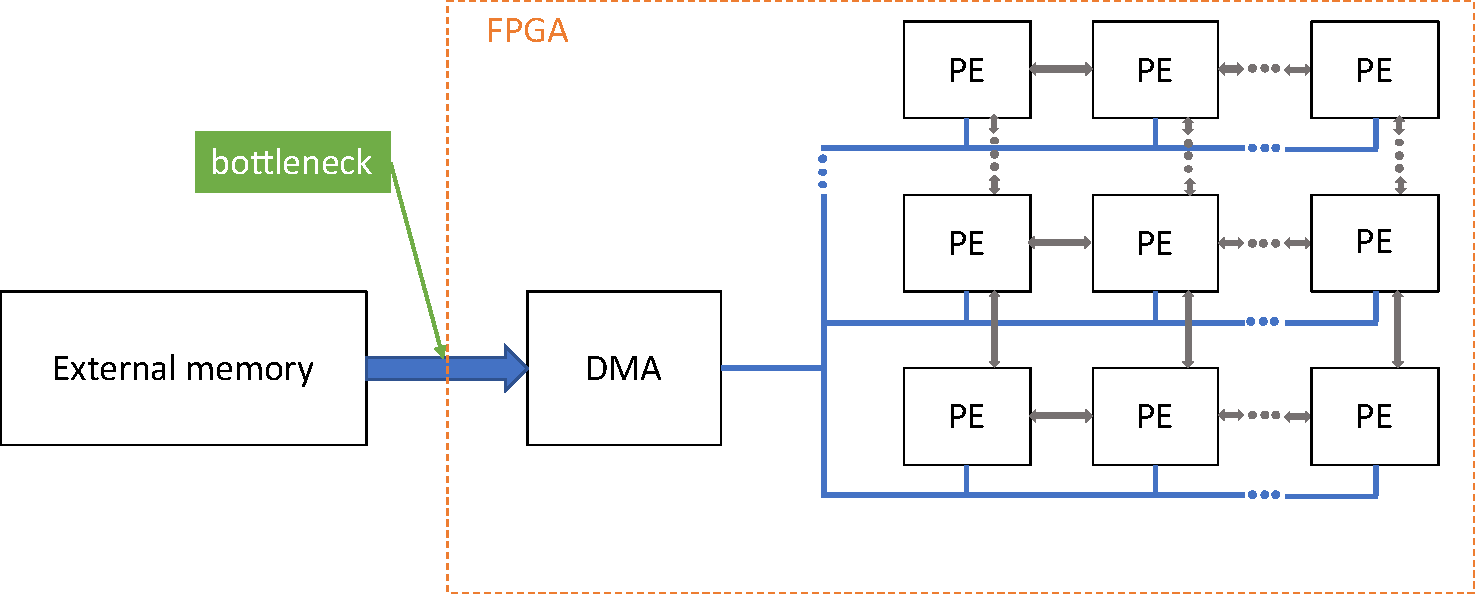
\includegraphics[width=\textwidth]{systArray.pdf}
    \caption{Static Systolic Arrays}
    \label{fig:sytar}
\end{figure}

However, Systolic Arrays has inefficiency problems. First, when the kernel size is much lesser than the maximal kernel size ($K_* << K_m$), there is an underutilization of the resources. For example, \cite{gokhale_240_2014} notes that for $3 \times 3$ kernels, only $9\%$ of the \acrfull{dsp} blocks are used. Second, data caching is not implemented. It means that it has always to fetch input from the external memory and it increases latency \cite{wei_automated_2017, abdelouahab_accelerating_2018}. The device performance is depending then on the memory bandwidth and it becomes memory-bounded. Furthermore, it is not energy efficient. According to \textcite{horowitz_11_2014}, the DRAM accesses severely impact both throughput and energy efficiency. DRAM accesses demand several orders of magnitude higher energy than computation.
%
%
\subsection{Data-flow MoC for CNNs (2D mapping)}
%
%
Data-flow \acrfull{moc} can be used to accelerate \acrshort{cnn}s on \acrshort{fpga}. This approach is motivated by the feed-forward aspect of the inference stage of \acrshort{cnn}, which is purely data-driven \cite{abdelouahab_accelerating_2018}. Data-flow \acrfull{moc} was firstly investigated by \cite{lin_li_low_2016}.  We can represent \acrshort{cnn} as a graph where:
\begin{itemize}
    \item \textbf{Nodes} are processing unit called an \textit{actor}. Each actor follows a data-driven execution where the execution is triggered by the availability of input, which is the case for a \acrshort{cnn}.
    \item \textbf{Edges} are communication \acrshort{fifo} channels. Actors exchange data called \textit{tokens} through those \acrshort{fifo} channels.
\end{itemize}
A representation of a such network can be found in Figure \ref{fig:moc}, where $FM_{*}^{i}$ is the ith layer of the \acrshort{fm}.

As the number of tokens produced and consumed by an actor can be specified in a \acrshort{cnn}, we can apply a static data-flow \cite{lee_static_1987}. The \acrshort{cnn} can be therefore modeled as a topology matrix and we only must, to minimize latency or energy consumption, optimize those matrix components (instead of tiling and unrolling parameters of section \ref{subsec:loopopti}) \cite{venieris_latency-driven_2017}. Those parameters are then used to derive \acrshort{pe} and buffer configurations. However, as pointed by \textcite{abdelouahab_tactics_2017}, we need to have a direct hardware mapping between the graph and the \acrshort{fpga} in order to be efficient. It means that all the computations must be unrolled. However, we are then bounded by the hardware resources and the size of the \acrshort{cnn}, preventing implementing this approach for deep models \cite{abdelouahab_accelerating_2018}.
\begin{figure}
    \centering
    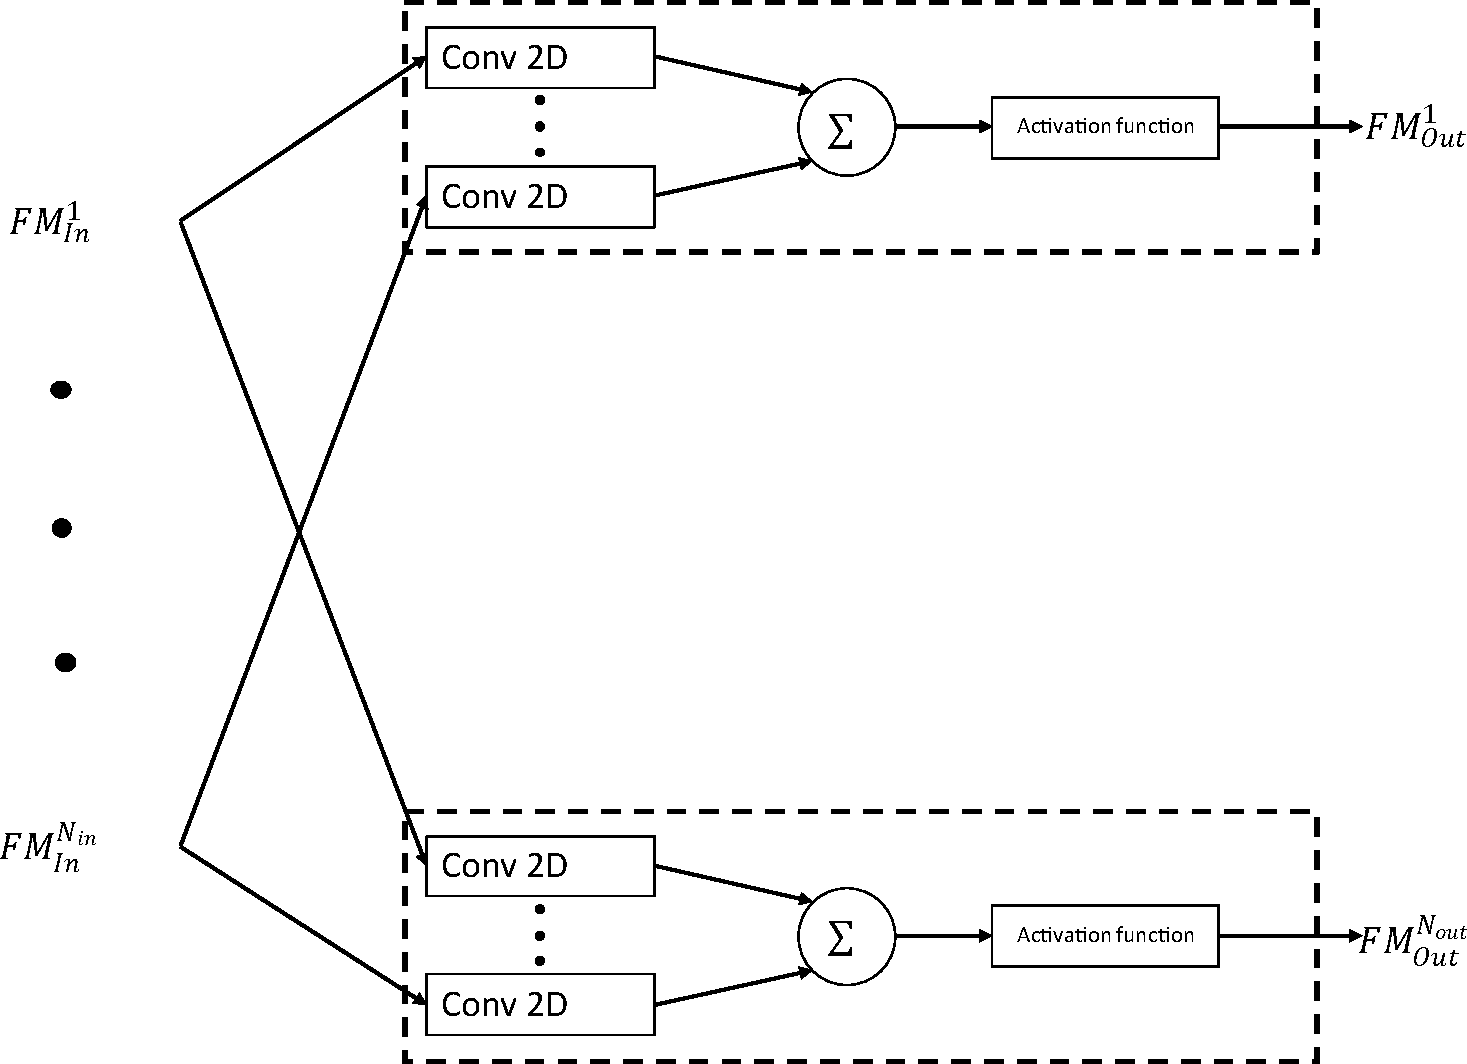
\includegraphics[width=0.8\textwidth]{Moc.pdf}
    \caption{Graph represenation of a convolution layer}
    \label{fig:moc}
\end{figure}
%
%
\subsection{Loop Optimizations} \label{subsec:loopopti}
%
%
To overcome the inefficiencies of Systollic arrays and because Data-flow \acrshort{moc} can only apply to small network, data must first be cached into the on-chip memory of the \acrshort{fpga} before processing. However, according to \textcite{ma_optimizing_2018}, the on-chip memory of \acrshort{fpga} is not enough to store all the data (requiring gigabytes). As a result, we need \textit{tiling} to fit a smaller portion of data into memory on-chip \cite{zhang_optimizing_2015}. We can summaryze the dataflow as follow: the \acrshort{fpga} fetches a tile of data from external memory to on-chip buffers. Then the data is fed to the \acrshort{pe}s to compute the convolution. The results of the computation is transferred back to on-chip buffers and aftewards, to external memory. When the results are written back to memory, we can fetch a new tile of data. We can see the process in Figure \ref{fig:hierarchy}

Consequently, we can define a storage hierarchy with different energy cost. We can define the memory levels as \cite{horowitz_11_2014, sze_efficient_2017}:
%
\begin{enumerate}
    \item \textbf{External Memory}: it stores all the \acrshort{cnn} data. It has a large memory capacity (\textasciitilde GB) but accesses are costly in terms of energy and latency.
    \item \textbf{On-chip buffers}: it stores the data fetched from external memory to feed the registers and \acrshort{pe}s. Accesses are less expensive with respect to the external memory but it has less storage (\textasciitilde hundreds of KB).
    \item \textbf{Registers}: it associated with the \acrshort{pe}s. The storage capacity is less than few KB but it is more faster and memory efficient. Accesses are 1 or 2 orders of magnitude lower energy than from DRAM.
\end{enumerate}
%
\begin{figure}
    \centering
    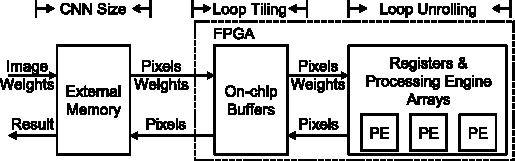
\includegraphics[width=\textwidth]{memhiera.pdf}
    \caption{\acrshort{fpga} memory hierarchy \cite{ma_optimizing_2018}}
    \label{fig:hierarchy}
\end{figure}

Therefore, after tiling, the convolution operation can be decomposed in multiple loops. We can observe the loop tiling in Figure \ref{fig:looptiling}. Nevertheless, an improper loop tiling may degrade performance of the \acrshort{fpga} because we must minimize access to expensive memory levels. Data reuse in small cost memories is then the major challenge when implementing a \acrshort{cnn} on \acrshort{fpga}. To address those problems, loop optimization techniques are applied to the nested loops in Figure \ref{fig:looptiling}. There are three techniques:
%
\begin{enumerate}
    \item \textbf{Loop tiling}: as said above, the on-chip memory of the \acrshort{fpga} is not enough to store all the weights and \acrshort{fm}s of all \acrshort{cnn} layers \cite{abdelouahab_accelerating_2018}. The \acrshort{fpga} stores a tile of the data, accessed from the external memory and the lower bound is set on the required on-chip buffer size. The tiling parameters represent the tile size. They are defined as: $T_{*}$, where $*$ is the name of the dimension. For example, the size of an input (resp. output) pixel buffer is $T_{ix} \times T_{iy} \times T_{if} \times $ pixel\_datawith ( $ T_{ox} \times T_{oy} \times T_{of} \times $ pixel\_datawith). Furthermore, we have the following constraint: $T_{*} \leq N_{*}$.
    \item \textbf{Loop interchange}: it defines the order of sequential computation of the computations loops. There are 2 types of loop interchange: \textit{intratile}, patterns of data movements from on-chip memory to registers (loop one to four in Figure \ref{fig:looptiling}); \textit{intertile}, patterns of data movements from external memory to on-chip buffers (the other loops).
    \item \textbf{Loop unrolling}: it determines the number of parallel computation. Four types of unrolling configuration can be done (depending on the loop to unroll). The different configurations can be seen in Figure \ref{fog:unroll}. As the \acrshort{fpga} has constrained resources, it is not always possible to fully unroll a loop. The unrolling parameters are defined as: $P_{*}$, where $*$ is the name of the dimension. We also have the following constraint: $P_{*} \leq T_{*} \leq N{*}$.
\end{enumerate}
%
\begin{figure}
\centering
\begin{lstlisting}[language=Java]
for (int of=0;of<N;of+=Tof){
  for (int iy=0;iy<Niy,iy+=Tiy){
    for (int ix=0;ix<Nix,ix+=Tix){
      for (int if=0;n<C;if+=Tif){
        // DRAM: Load in on chip buffers the tiles
        // X[l,if:if+Tif,iy:iy+Ty,ix:ix+Tix]
        // Theta [l,n:n+Tof,if:if+Tif,j,k]
          for (int tof=0;tof<Tof;tof++){ -> Loop-4
            for (int tiy=0;tiy<Tiy,tiy++){ -> Loop-3
              for (int tix=0;tix<Tix,tix++){ -> Loop-3
                for (int tif=0;tof<Tif;tif++){ -> Loop-2
                  for (int ky=0;ky<Nky,ky++){ -> Loop-1
                    for (int kx=0;kx<Nkx,kx++){ -> Loop-1
                      Y[tof,tiy,tix] += X[tif,tiy+ky,tix+kx] *
                      W[tof,tif,ky,kx];
          }}}}}}
          // DRAM: Store output tile
}}}}
    \end{lstlisting}
    \caption{Loop Tiling, from \cite{abdelouahab_accelerating_2018}}
    \label{fig:looptiling}
\end{figure}
%
\begin{figure}
    \centering
    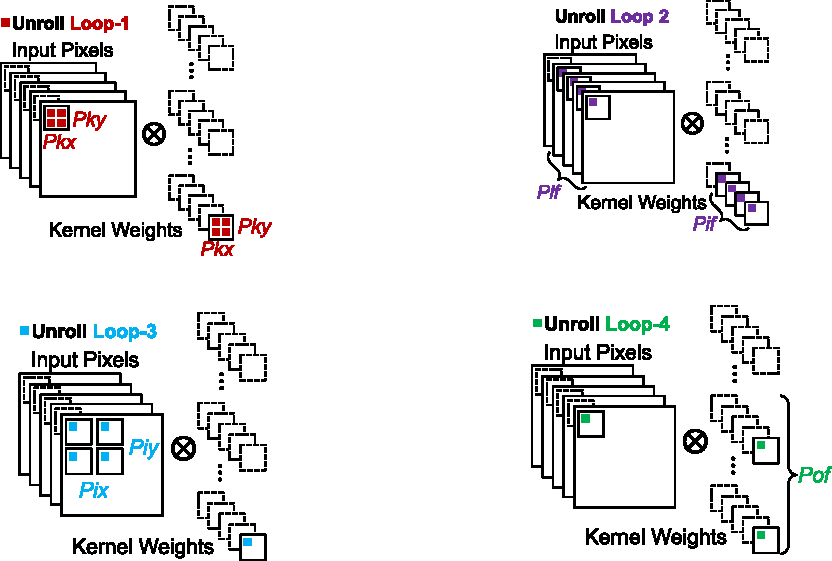
\includegraphics[width=\textwidth]{unroll.pdf}
    \caption{Loop unrolling configurations \cite{ma_optimizing_2018}}
    \label{fog:unroll}
\end{figure}

The loop optimization design variables determine the number of \acrshort{pe}s, the buffer size and the number of external memory access. We are going to review different works who study the design space exploration of unrolling parameters, tiling parameters, and loop interchange, to design the most efficient accelerator that would be feasible on the target platform.

The work of \textcite{zhang_optimizing_2015} proposes an analytical solution using the roofline model \cite{williams_roofline_2009} to identify the CNN design with the best performance and lowest \acrshort{fpga} resource requirement. They have chosen a loop unrolling of ($T_{if} \times T_{of}$) to avoid complex connection topologies for all arrays. It allows spatial reuse of pixels for $T_{of}$ unrolls, and the temporal reuse of weight for ($T_{ox} \times T_{oy}$). However, the disadvantage of this method is the need for a large local memory to store the partial sums ($T_{of} \times T_{ox} \times T_{oy}$).

Once the loop ordering and unrolling parameters have been set, the roofline model can be used to find the optimal tiling parameters. \textcite{mittal_survey_2020} defines this design space exploration method as: \textquote{\textit{The roofline model relates performance to computational performance and off-chip memory traffic}}. As an implementation can either be computation-bounded or memory-bounded, it uses those two limits to find the best trade-off between memory bandwidth and computational speed.
\begin{enumerate}
    \item \textbf{Computational roof}: $= \frac{\text{\# \ of \ operations}}{\# \ of \ execution \ cycles}$.
    \item \textbf{CTC ratio}: $= \frac{\text{\# \ of \ operations}}{\# \ of \ external \ data \ access}$
\end{enumerate}
Therefore, we can compute the attainable performance as equation \ref{eq:atperf}.
\begin{equation}
Att \ perf = min \ (Computational \ roof; CTC \ ratio \times bandwidth)
\label{eq:atperf}
\end{equation}

The roofline method is shown in Figure \ref{fig:roofmeth}. In this figure, implementations C and D achieves the highest possible performance on the \acrshort{fpga}. However, implementation C is preferred because it requires the least bandwidth.
%
\begin{figure}
    \centering
    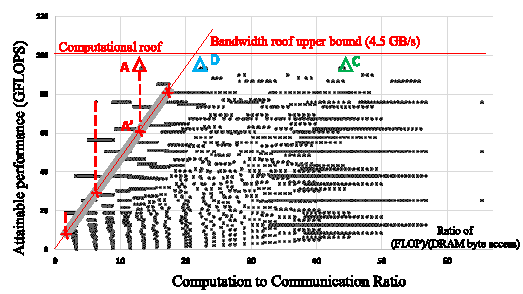
\includegraphics[width=\textwidth]{roofmethod.pdf}
    \caption{Design space of platform-supported designs  \cite{zhang_optimizing_2015}}
    \label{fig:roofmeth}
\end{figure}

\textcite{motamedi_placid_2017} chooses the best parameters according to its resources and the data reuse scheme. They do not tile on the kernel and on the spatial axis because the on-chip memory is larger than an \acrshort{fm} size and recent \acrshort{cnn} have small filters, and to avoid the problem of loading multiple times the same pixel. As the tile goes over the input and output \acrshort{fm} channel, we can choose between maximizing the reuse of the input \acrshort{fm} (MIR, each \acrshort{fm} is loaded once but some intermediate results have to be wrote back to memory) or output \acrshort{fm} (MOR, we avoid writing back intermediate results to memory but some input \acrshort{fm} have to be loaded more than once). Then they perform an exhaustive search on the tiling and \acrshort{pe} parameters to find the optimal design. It can be layer-specific (but the \acrshort{fpga} needs dynamic reconfiguration and \textcite{zhang_optimizing_2015} have proven it is inefficient) or values are fixed for all layer.

A different approach, studied by \textcite{ma_optimizing_2018}, proposes a design space exploration regarding various design objectives. They have proposed two flowcharts in Figure \ref{fig:flowchart} to
\begin{itemize}
    \item \textbf{Latency}: $P_*$ should be common factors of  $T_*$ for all convolution layers to fully utilize \acrshort{pe}s, and $T_*$ to be the common factors of  $N_*$ to make full use of external memory transactions.
    \item \textbf{Partial sum storage}: to minimize the concurrent storage of partial sums in local memory and allowing to keep them into the PE, we should prior the computation of an output pixel to evacuate it to the external memory.
    \item \textbf{On-chip memory access}: on-chip memory access can be minimized by reusing at most pixels or weights in the \acrshort{pe}s.
    \item \textbf{External memory access}: to minimize external access, a sufficient buffer size should be assigned to pixels and weights.
\end{itemize}
%
\begin{figure}
\centering
    \begin{subfigure}{.45\textwidth}
    \centering
    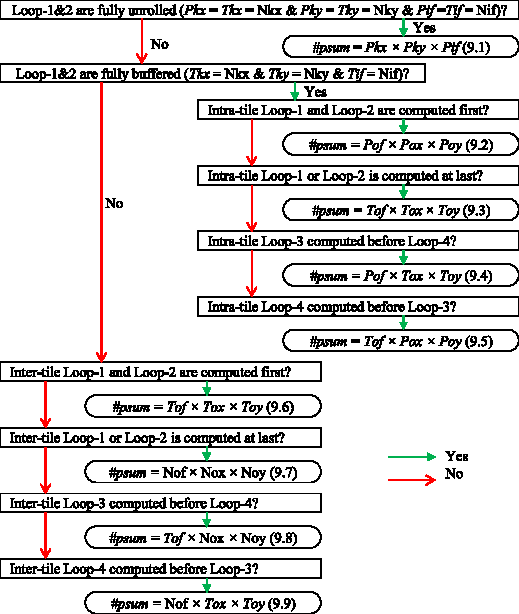
\includegraphics[width=\linewidth]{fwch1.pdf}
    \caption{ }
    \end{subfigure}
    \begin{subfigure}{.45\textwidth}
    \centering
    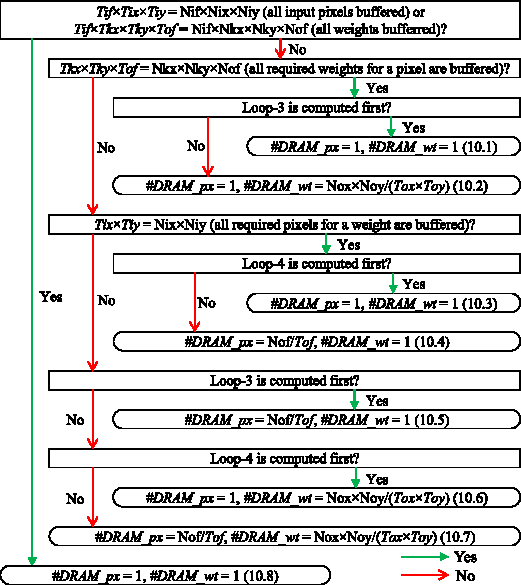
\includegraphics[width=\linewidth]{fwch2.pdf}
    \caption{ }
    \end{subfigure}
    \caption{Design space exploration of: (a) total number of partial sums that need to be stored in memory; (b) the number of external memory accesses \cite{ma_optimizing_2018}}
    \label{fig:flowchart}
\end{figure}
